
\documentclass[paper=a4, fontsize=11pt]{scrartcl} % A4 paper and 11pt font size

\usepackage[T1]{fontenc} % Use 8-bit encoding that has 256 glyphs
\usepackage{fourier} % Use the Adobe Utopia font for the document - comment this line to return to the LaTeX default
\usepackage[english]{babel} % English language/hyphenation
\usepackage{amsmath,amsfonts,amsthm} % Math packages

\usepackage{graphicx}
\usepackage{hyperref}
\usepackage{csvsimple}

\usepackage{verbatim}

\usepackage{sectsty} % Allows customizing section commands
%\allsectionsfont{\centering \normalfont\scshape} % Make all sections centered, the default font and small caps

\usepackage{fancyhdr} % Custom headers and footers
\usepackage{listings}
\usepackage{color}
\usepackage[T1]{fontenc}

\definecolor{dkgreen}{rgb}{0,0.6,0}
\definecolor{gray}{rgb}{0.5,0.5,0.5}
\definecolor{mauve}{rgb}{0.58,0,0.82}

\lstset{frame=tb,
  language=Python,
  aboveskip=3mm,
  belowskip=3mm,
  showstringspaces=false,
  columns=flexible,
  basicstyle={\small\ttfamily},
  numbers=none,
  numberstyle=\tiny\color{gray},
  keywordstyle=\color{blue},
  commentstyle=\color{dkgreen},
  stringstyle=\color{mauve},
  breaklines=true,
  breakatwhitespace=true,
  tabsize=3
}
\newcommand{\subf}[2]{%
  {\small\begin{tabular}[t]{@{}c@{}}
  #1\\#2
  \end{tabular}}%
}

\pagestyle{fancyplain} % Makes all pages in the document conform to the custom headers and footers
\fancyhead{} % No page header - if you want one, create it in the same way as the footers below
\fancyfoot[L]{} % Empty left footer
\fancyfoot[C]{} % Empty center footer
\fancyfoot[R]{\thepage} % Page numbering for right footer
\renewcommand{\headrulewidth}{0pt} % Remove header underlines
\renewcommand{\footrulewidth}{0pt} % Remove footer underlines
\setlength{\headheight}{13.6pt} % Customize the height of the header

\numberwithin{equation}{section} % Number equations within sections (i.e. 1.1, 1.2, 2.1, 2.2 instead of 1, 2, 3, 4)
\numberwithin{figure}{section} % Number figures within sections (i.e. 1.1, 1.2, 2.1, 2.2 instead of 1, 2, 3, 4)
\numberwithin{table}{section} % Number tables within sections (i.e. 1.1, 1.2, 2.1, 2.2 instead of 1, 2, 3, 4)

\setlength\parindent{0pt} % Removes all indentation from paragraphs - comment this line for an assignment with lots of text

%----------------------------------------------------------------------------------------
%	TITLE SECTION
%----------------------------------------------------------------------------------------

\newcommand{\horrule}[1]{\rule{\linewidth}{#1}} % Create horizontal rule command with 1 argument of height

\title{	
\normalfont \normalsize 
\textsc{Indraprastha Institute of Information Technology, Delhi} \\ [25pt] % Your university, school and/or department name(s)
\horrule{0.5pt} \\[0.4cm] % Thin top horizontal rule
\huge Homework 1 : Twitter and FB data analysis\\ % The assignment title
\horrule{2pt} \\[0.5cm] % Thick bottom horizontal rule
}

\author{Sagar Verma} % Your name

\date{\normalsize\today} % Today's date or a custom date

\begin{document}


\maketitle % Print the TI


%\csvautotabular[respect all]{cercwww.csv}

\subsection{CERCatIIITD \#posts vs time}
Below graph shows Number of Posts for each month from creating of page till the date data was collected.
21 posts were obtained from CERCatIIITD page which contain What, Where and When in thier description.\\
\begin{center}
  \makebox[\textwidth]{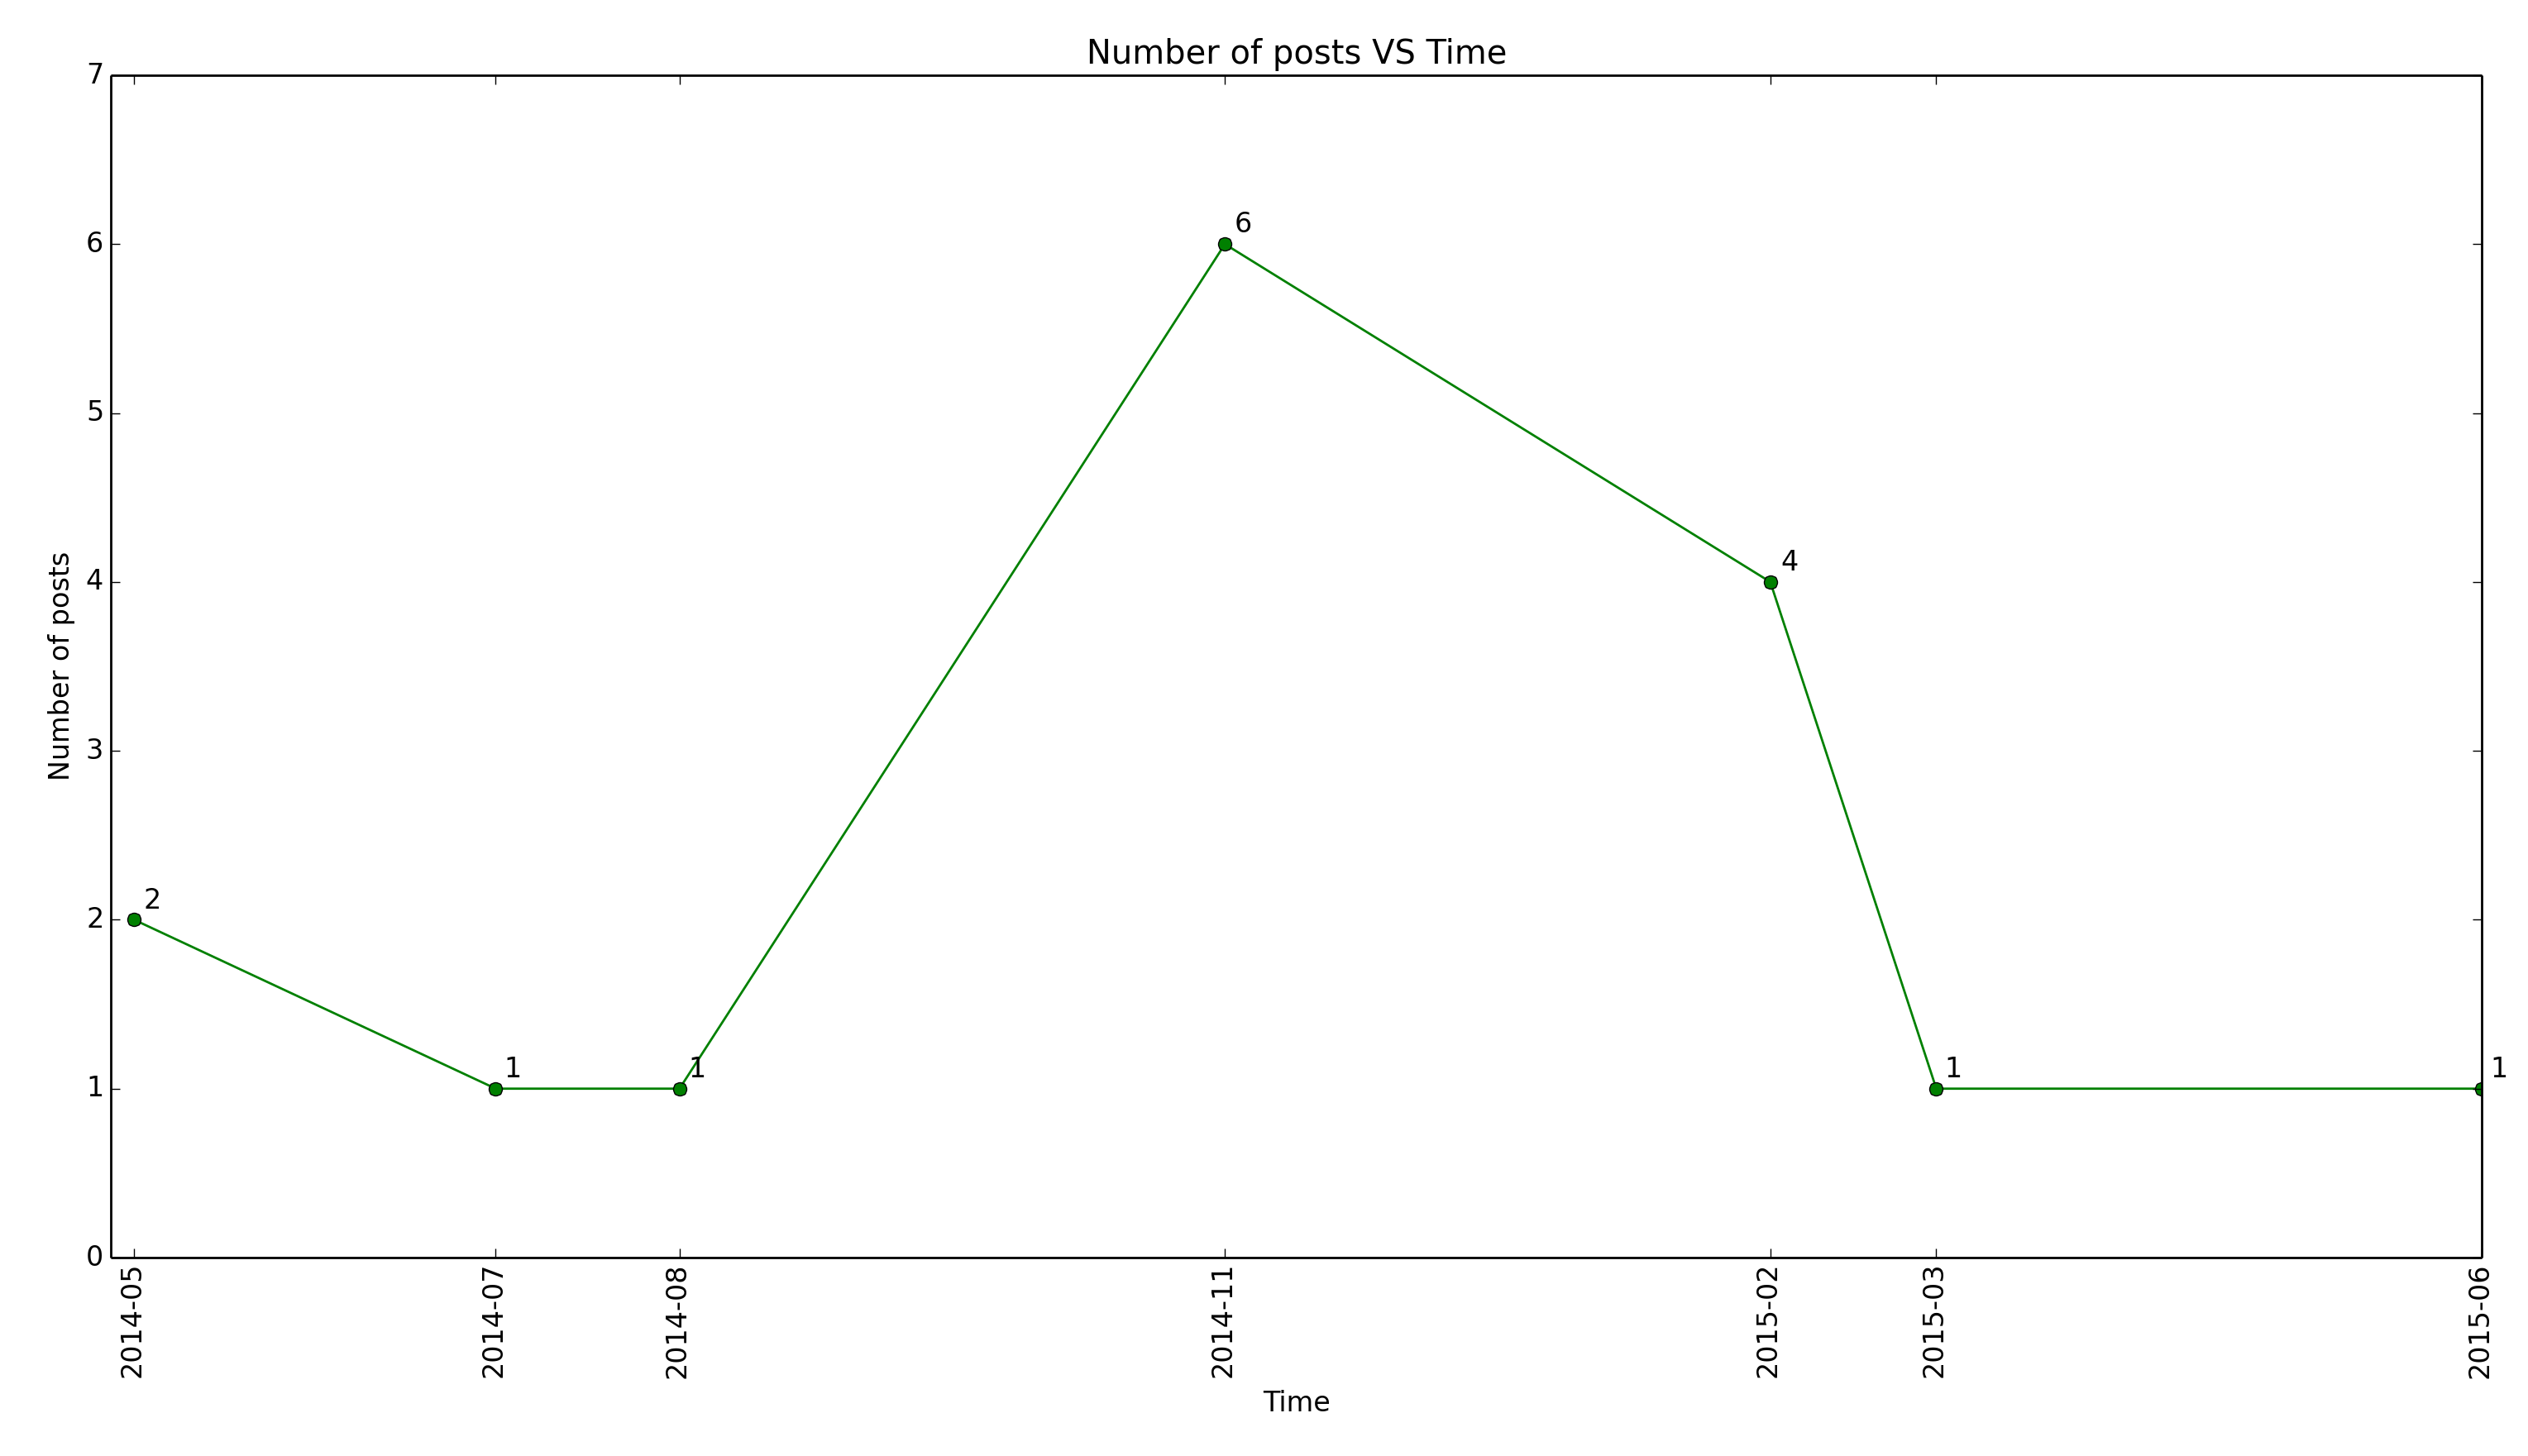
\includegraphics[width=550px, height=250px]{cerc_year}}
\end{center}
\newpage
\subsection{CERCatIIITD word cloud}
Now, for the given graph we create a word cloud for the month page was created, for months which the number of posts are high and for the end of the month. Here they are "2014-05","2014-11","2015-03","2015-06".
\begin{figure}[!htb]
\centering
\begin{tabular}{|c|c|}
\hline
\subf{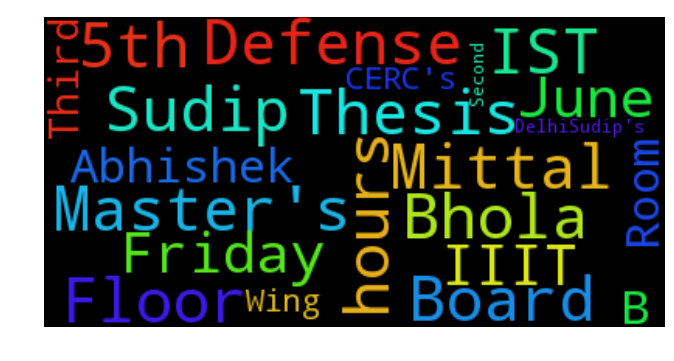
\includegraphics[width=180px]{cerc2014-05_word_cloud_rel}}
     {CERCatIIITD Words used during May, 2014}
&
\subf{
\includegraphics[width=180px]{cerc2014-11_word_cloud_rel}}
     {CERCatIIITD Words used during Nov, 2014}
\\
\hline
\subf{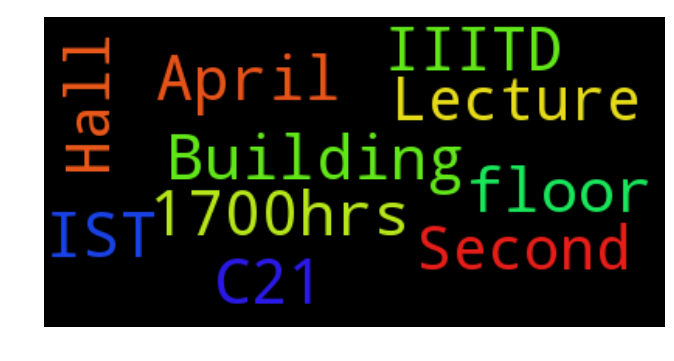
\includegraphics[width=180px]{cerc2015-03_word_cloud_rel}}
     {CERCatIIITD Words used during March, 2015}
&
\subf{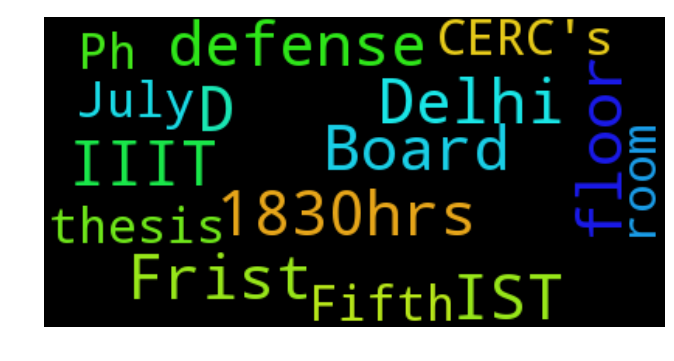
\includegraphics[width=180px]{cerc2015-06_word_cloud_rel}}
     {CERCatIIITD Words used during June, 2015}
\\
\hline
\end{tabular}
\end{figure}

From word cloud we see that the page is talking mostly about  CERC building, reading,  thesis defense and \href{https://www.facebook.com/ponnurangam.kumaraguru/media_set?set=a.944918412200139.1073741872.100000459677395&type=1&l=7cbb458dff}{symposium}.\\

\newpage
\subsection{blrcitypolice \#posts vs time}
For Banglore city police facebook page, we draw word clouds for"2012-08","2015-01","2015-03","2015-08".
14348 posts were extracted from blrcitypolice page.\\

\begin{center}
  \makebox[\textwidth]{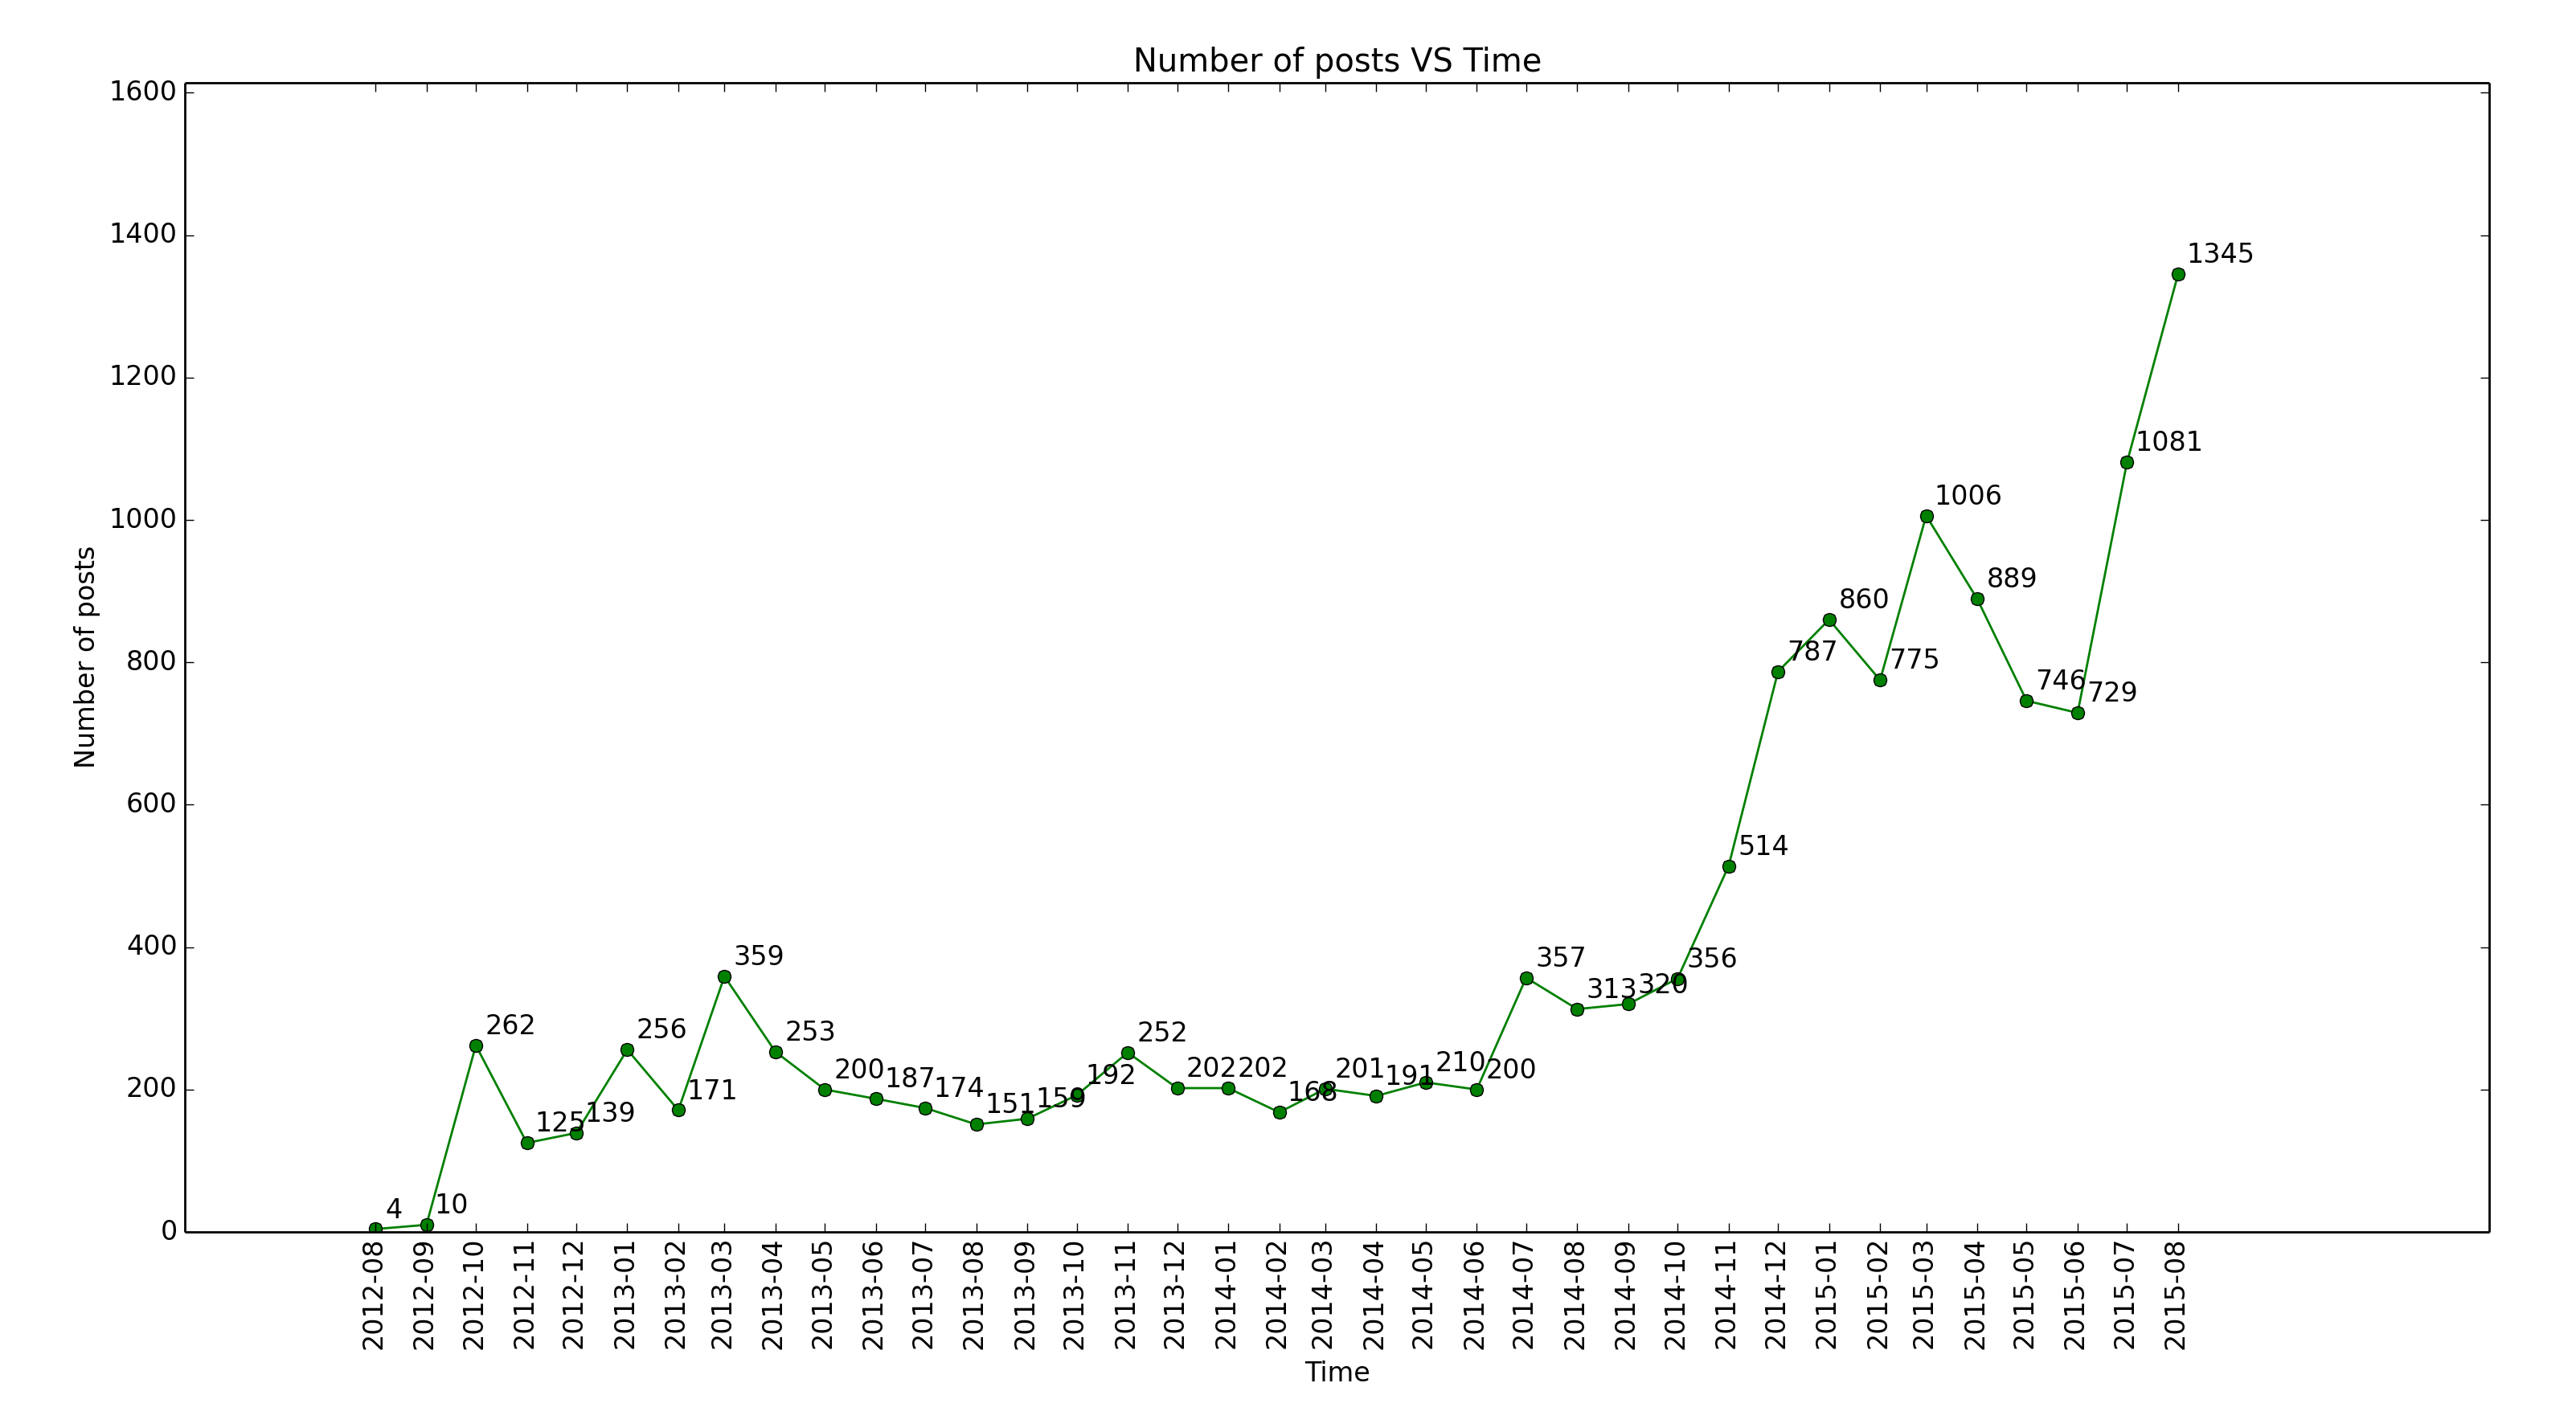
\includegraphics[width=550px, height=310px]{blrcitypolice_year}}
\end{center}
\newpage
\subsection{blrcitypolicei word cloud}
\begin{figure}[!htb]
\centering
\begin{tabular}{|c|c|}
\hline
\subf{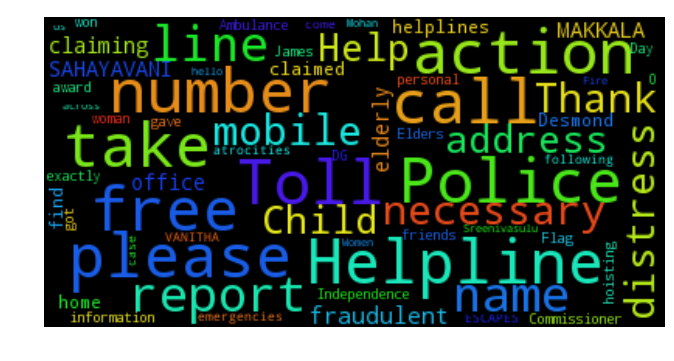
\includegraphics[width=180px]{blrcitypolice2012-08_word_cloud_rel}}
     {blrcitypolice Words used during August, 2012}
&
\subf{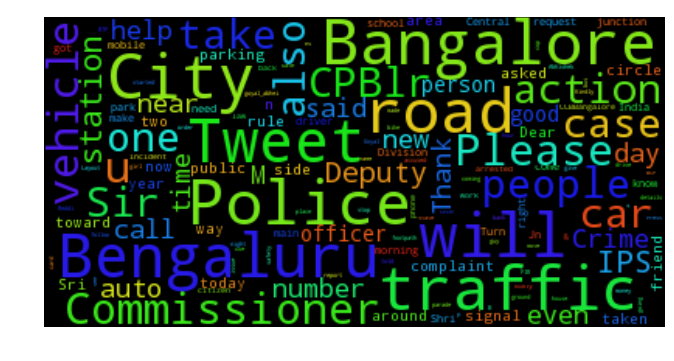
\includegraphics[width=180px]{blrcitypolice2015-01_word_cloud_rel}}
     {blrcitypolice Words used during Janurary, 2014}
\\
\hline
\subf{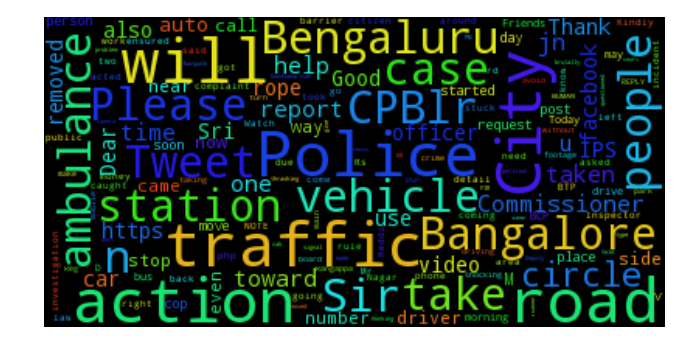
\includegraphics[width=180px]{blrcitypolice2015-03_word_cloud_rel}}
     {blrcitypolice Words used during March, 2015}
&
\subf{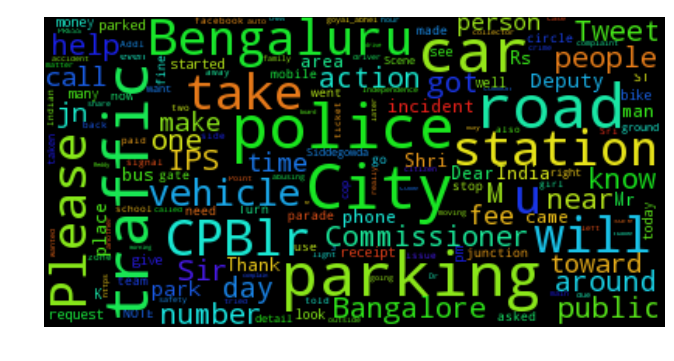
\includegraphics[width=180px]{blrcitypolice2015-08_word_cloud_rel}}
     {blrcitypolice Words used during August, 2015}
\\
\hline
\end{tabular}
\end{figure}
Most posts are about Bangalore road safety and traffics.\\
Most posts are by random people asking Commisoner of Police regarding road safety and other law and order related tasks.\href{https://fbstatic-a.akamaihd.net/rsrc.php/v2/y4/r/-PAXP-deijE.gif}{A post of real time crime}.\\
On careful analysis of each date by manuaaly reading the twitter data of March-August 2015, the people are talking about \href{http://www.newindianexpress.com/states/karnataka/Social-Media-Seeks-Justice-for-Ravi/2015/03/18/article2719047.ece} {IAS DK Ravi's case}.

\newpage
\subsection{ponguru \#posts vs time}
For ponguru tweeter handle, we draw the word cloud for spikes present in the time series graph, i.e., "2011-04","2013-03","2014-02","2015-07".
1017 records were found for ponguru twitter handle.\\
\begin{center}
  \makebox[\textwidth]{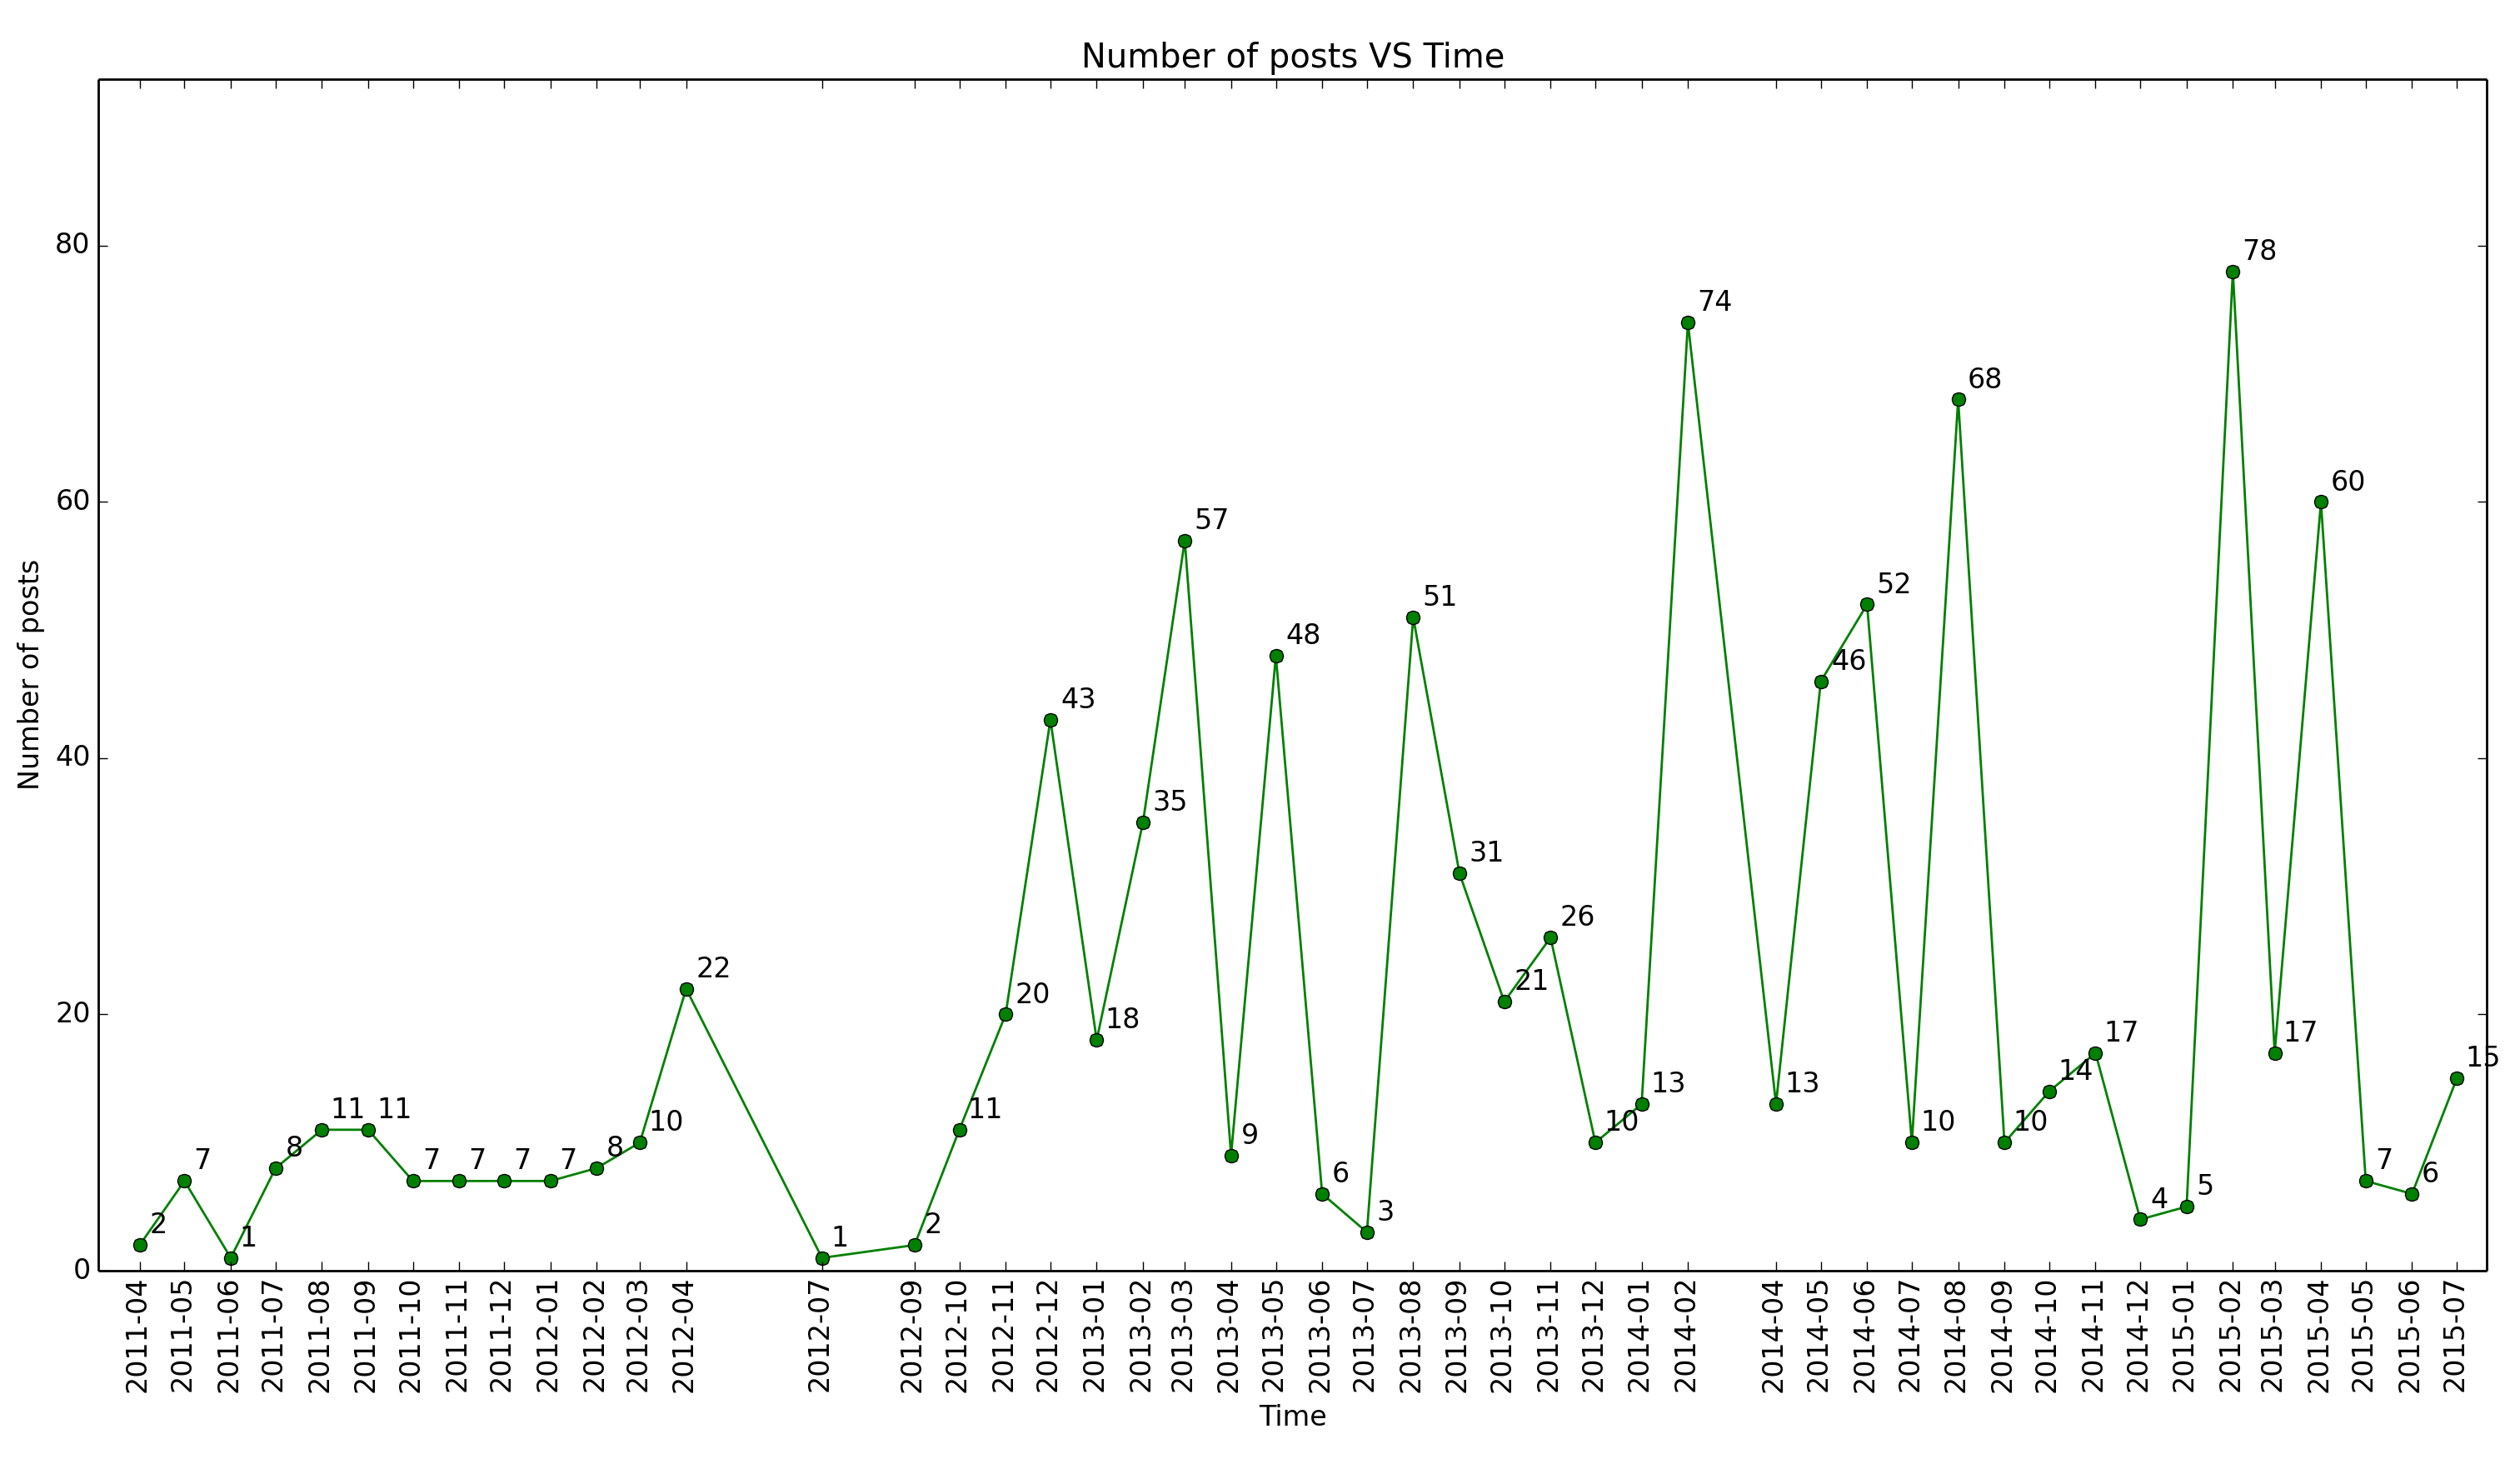
\includegraphics[width=550px, height=310px]{ponguru_year}}
\end{center}
\newpage
\subsection{ponguru word cloud}
\begin{figure}[!htb]
\centering
\begin{tabular}{|c|c|}
\hline
\subf{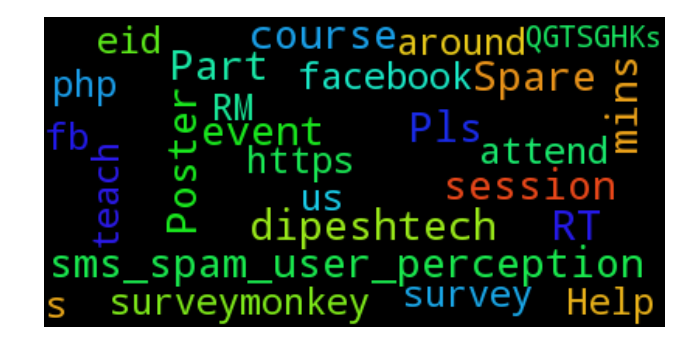
\includegraphics[width=180px]{ponguru2011-04_word_cloud_rel}}
     {ponguru Words used during April, 2011}
&
\subf{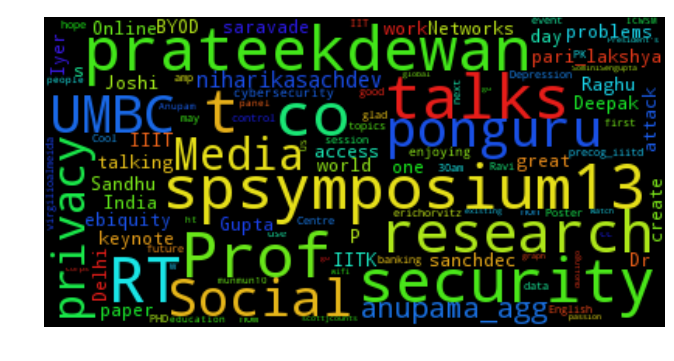
\includegraphics[width=180px]{ponguru2013-03_word_cloud_rel}}
     {ponguru Words used during March, 2013}
\\
\hline
\subf{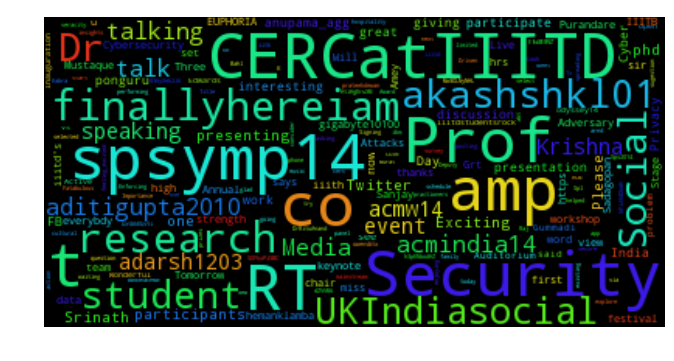
\includegraphics[width=180px]{ponguru2014-02_word_cloud_rel}}
     {ponguru Words used during Feburary, 2014}
&
\subf{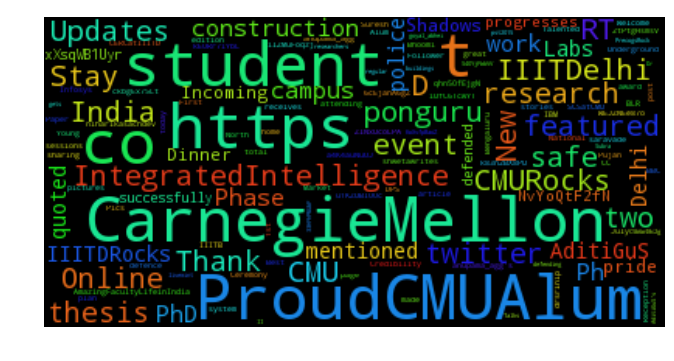
\includegraphics[width=180px]{ponguru2015-07_word_cloud_rel}}
     {ponguru Words used during July, 2015}
\\
\hline
\end{tabular}
\end{figure}
Tweets are about Security \href{https://twitter.com/hashtag/spsymp15?src=hash}{simposium} 2013,2014 and 2015.
\newpage
\subsection{thekiranbedi \#posts vs time}
For thekiranbedi twitter handle, we make the word clouds for month ID was created, month data was collected and two months in between were there were maximum \#posts, i.e. "2014-11","2015-05","2015-07","2015-08".
3247 tweets were extracted from thekiranbedi twitter handle.\\
Data limit for Facebook is 320 per request and one can get all posts of an ID and for Twitter it is arround 3300 per ID.\\
\begin{center}
  \makebox[\textwidth]{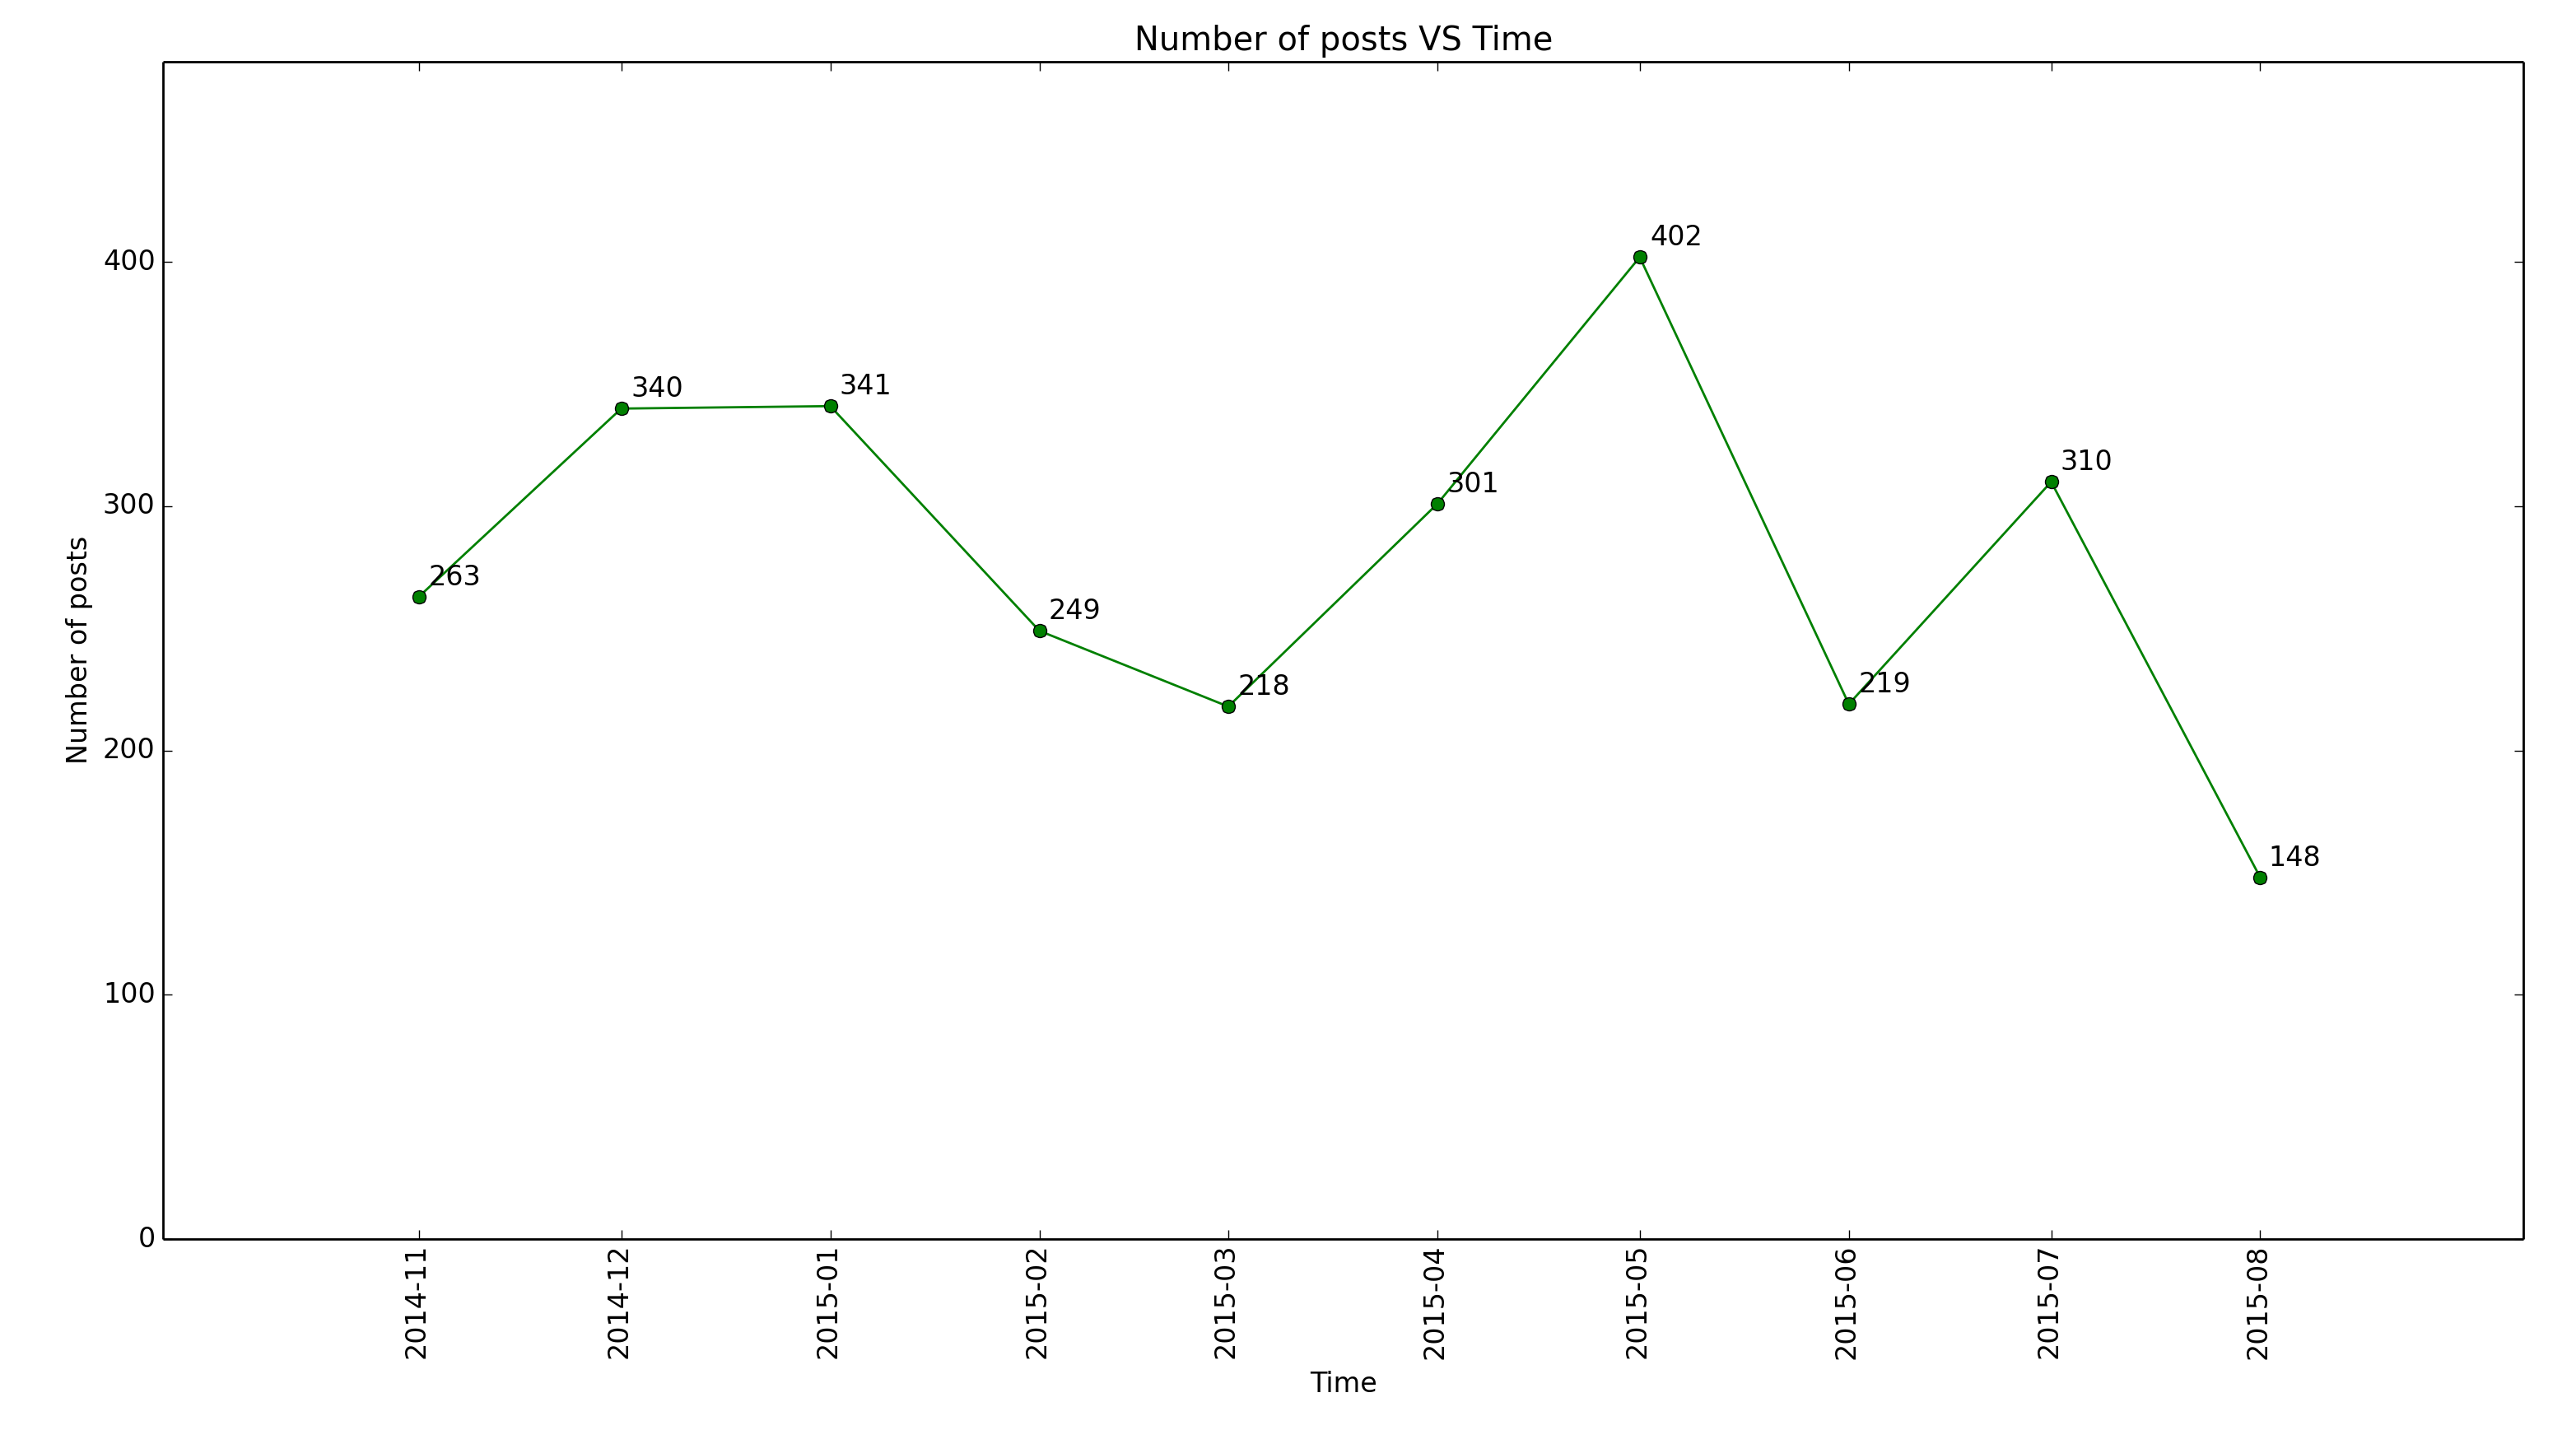
\includegraphics[width=550px, height=310px]{thekiranbedi_year}}
\end{center}
The graph for thekiranbedi handle is much denser then ponguru and CERCatIIITD, this shows that thekiranbedi's user is more active. blrcitypolice has maximum number of posts and about 80\% of those are posts by page followers.\\
\newpage
\subsection{thekiranbedi word cloud}
\begin{figure}[!htb]
\centering
\begin{tabular}{|c|c|}
\hline
\subf{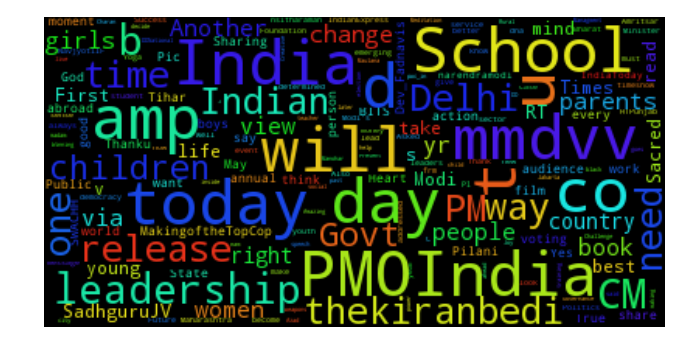
\includegraphics[width=180px]{thekiranbedi2014-11_word_cloud_rel}}
     {thekiranbedi Words used during November, 2014}
&
\subf{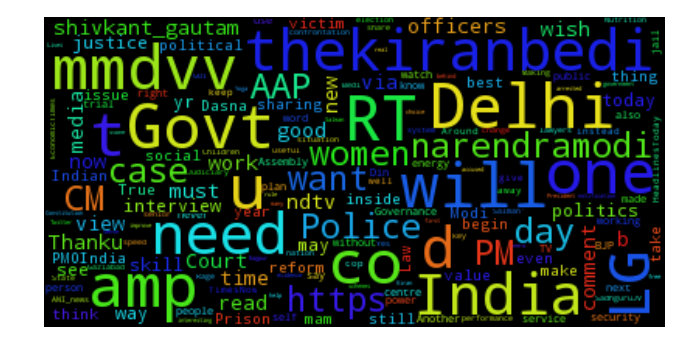
\includegraphics[width=180px]{thekiranbedi2015-05_word_cloud_rel}}
     {thekiranbedi Words used during May, 2015}
\\
\hline
\subf{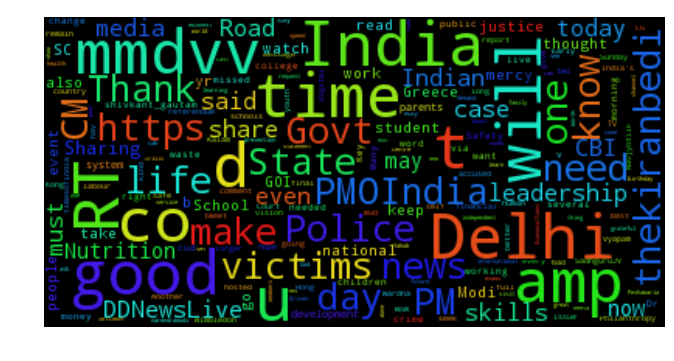
\includegraphics[width=180px]{thekiranbedi2015-07_word_cloud_rel}}
     {thekiranbedi Words used during July, 2015}
&
\subf{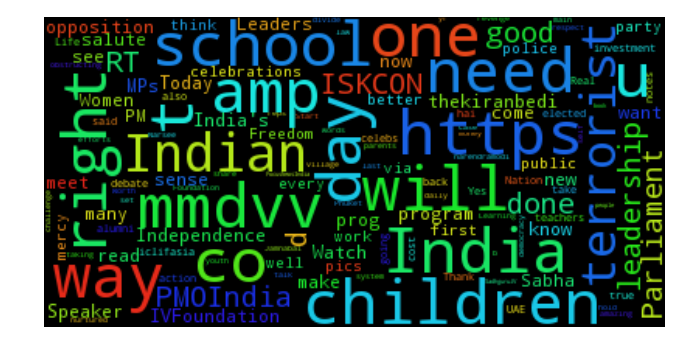
\includegraphics[width=180px]{thekiranbedi2015-08_word_cloud_rel}}
     {thekiranbedi Words used during August, 2015}
\\
\hline
\end{tabular}
\end{figure}
Tweets are realated to AAP, BJP, PMO India and \href{https://twitter.com/thekiranbedi/status/633106539130175488}{Women and Child welfare}.
\newpage
\subsection{Word clouds of all the IDs showing frequent words used by IDs}
Word cloud showing what each ID's have talked about most from the time ID was created till last time data was collected.\\
\begin{figure}[!htb]
\centering
\begin{tabular}{|c|c|}
\hline
\subf{
\includegraphics[width=180px]{cerc_word_cloud_rel}}
     {CERCatIIITD : Frequent words in whole page.}
&
\subf{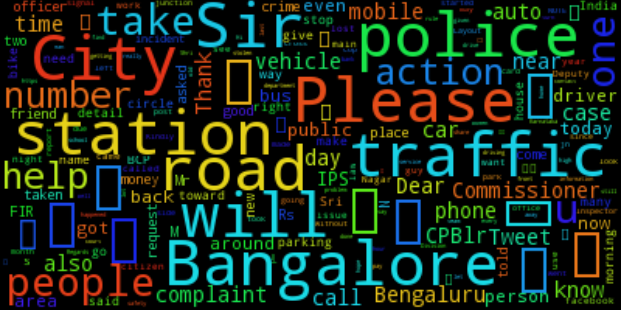
\includegraphics[width=180px]{blrcitypolice_word_cloud_rel}}
     {blrcitypolice : Frequent words in whole page.}
\\
\hline
\subf{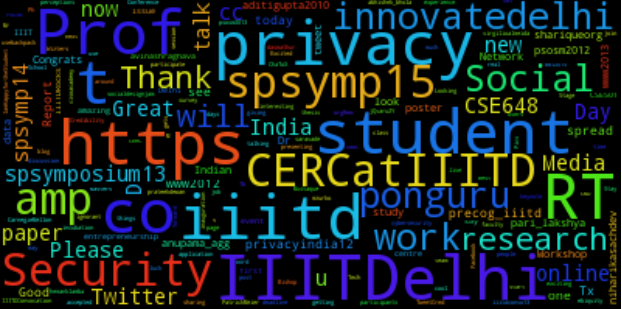
\includegraphics[width=180px]{ponguru_word_cloud_rel}}
     {ponguru : Frequent words in all the tweets.}
&
\subf{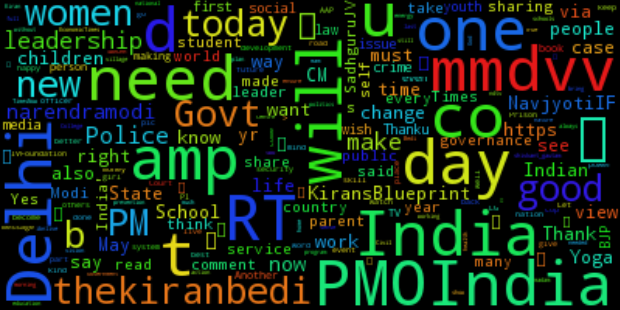
\includegraphics[width=180px]{thekiranbedi_word_cloud_rel}}
     {thekiranbedi : Frequent word in all the tweets.}
\\
\hline
\end{tabular}
\end{figure}

\newpage
\subsection{Sentiment scores vs time for all IDs}
The following graphs show sentiments of IDs with time. Since API provides very less data daily only few data was collected. If we carefully analyse the tweets for which the sentiment score is very high -ve or +ve we can find the reason behind the score.\\
\\
blrcitypolice(Banglore City Police)
\begin{center}
 \makebox[\textwidth]{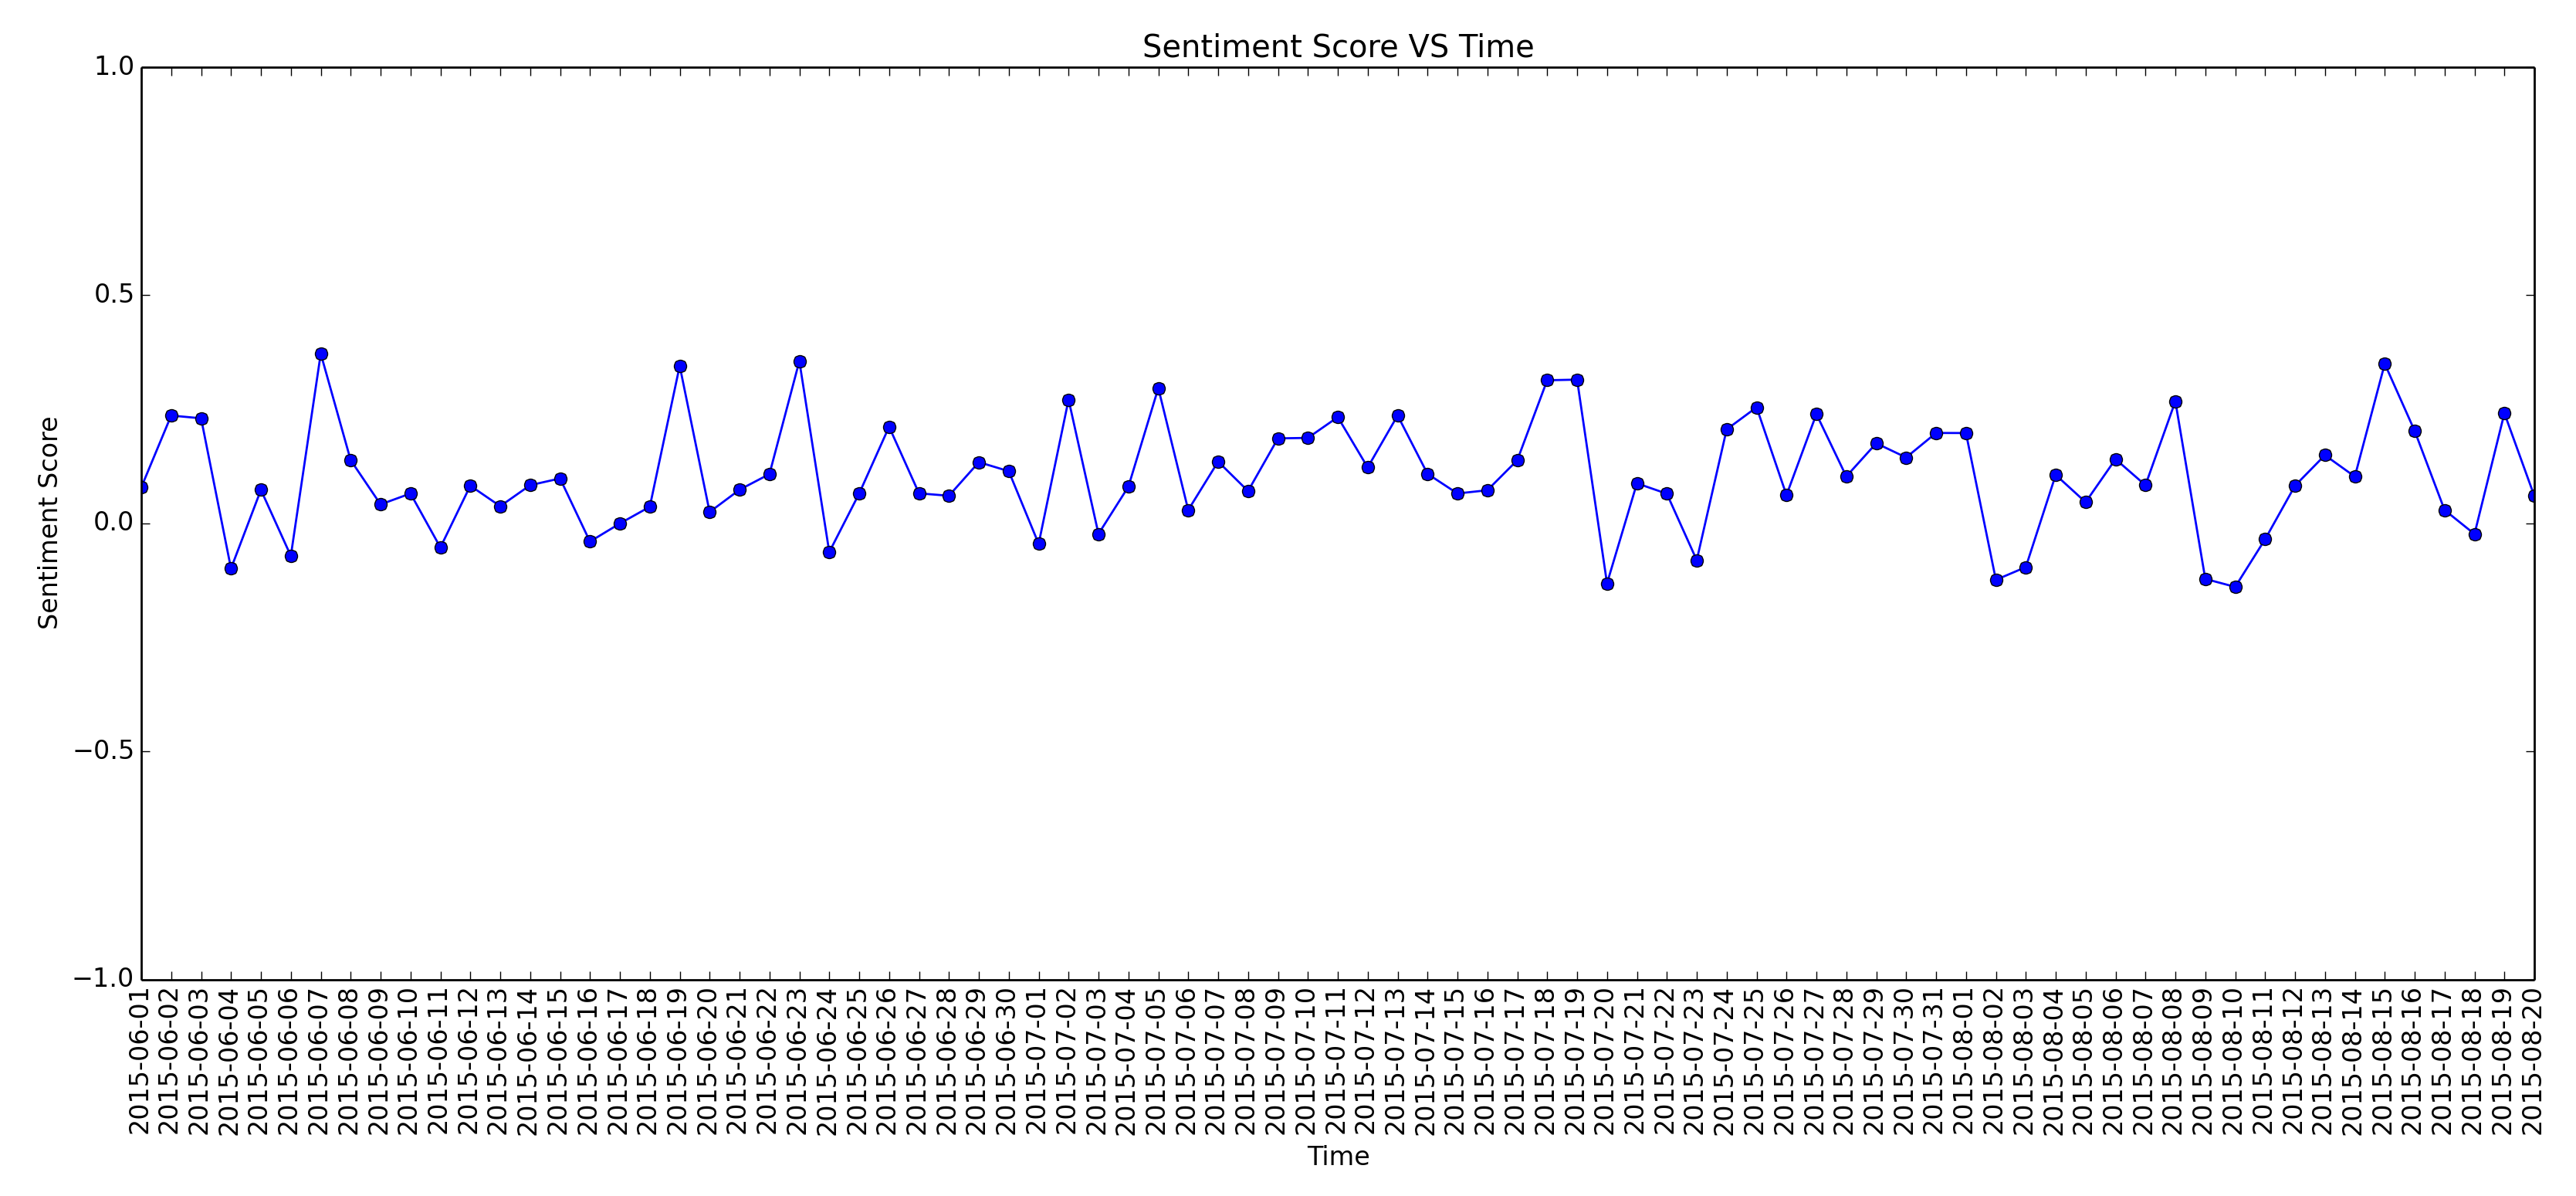
\includegraphics[width=550px, height=310px]{blrcitypolice_senti_time}}
\end{center}
\newpage
ponguru(PK)
\begin{center}
 \makebox[\textwidth]{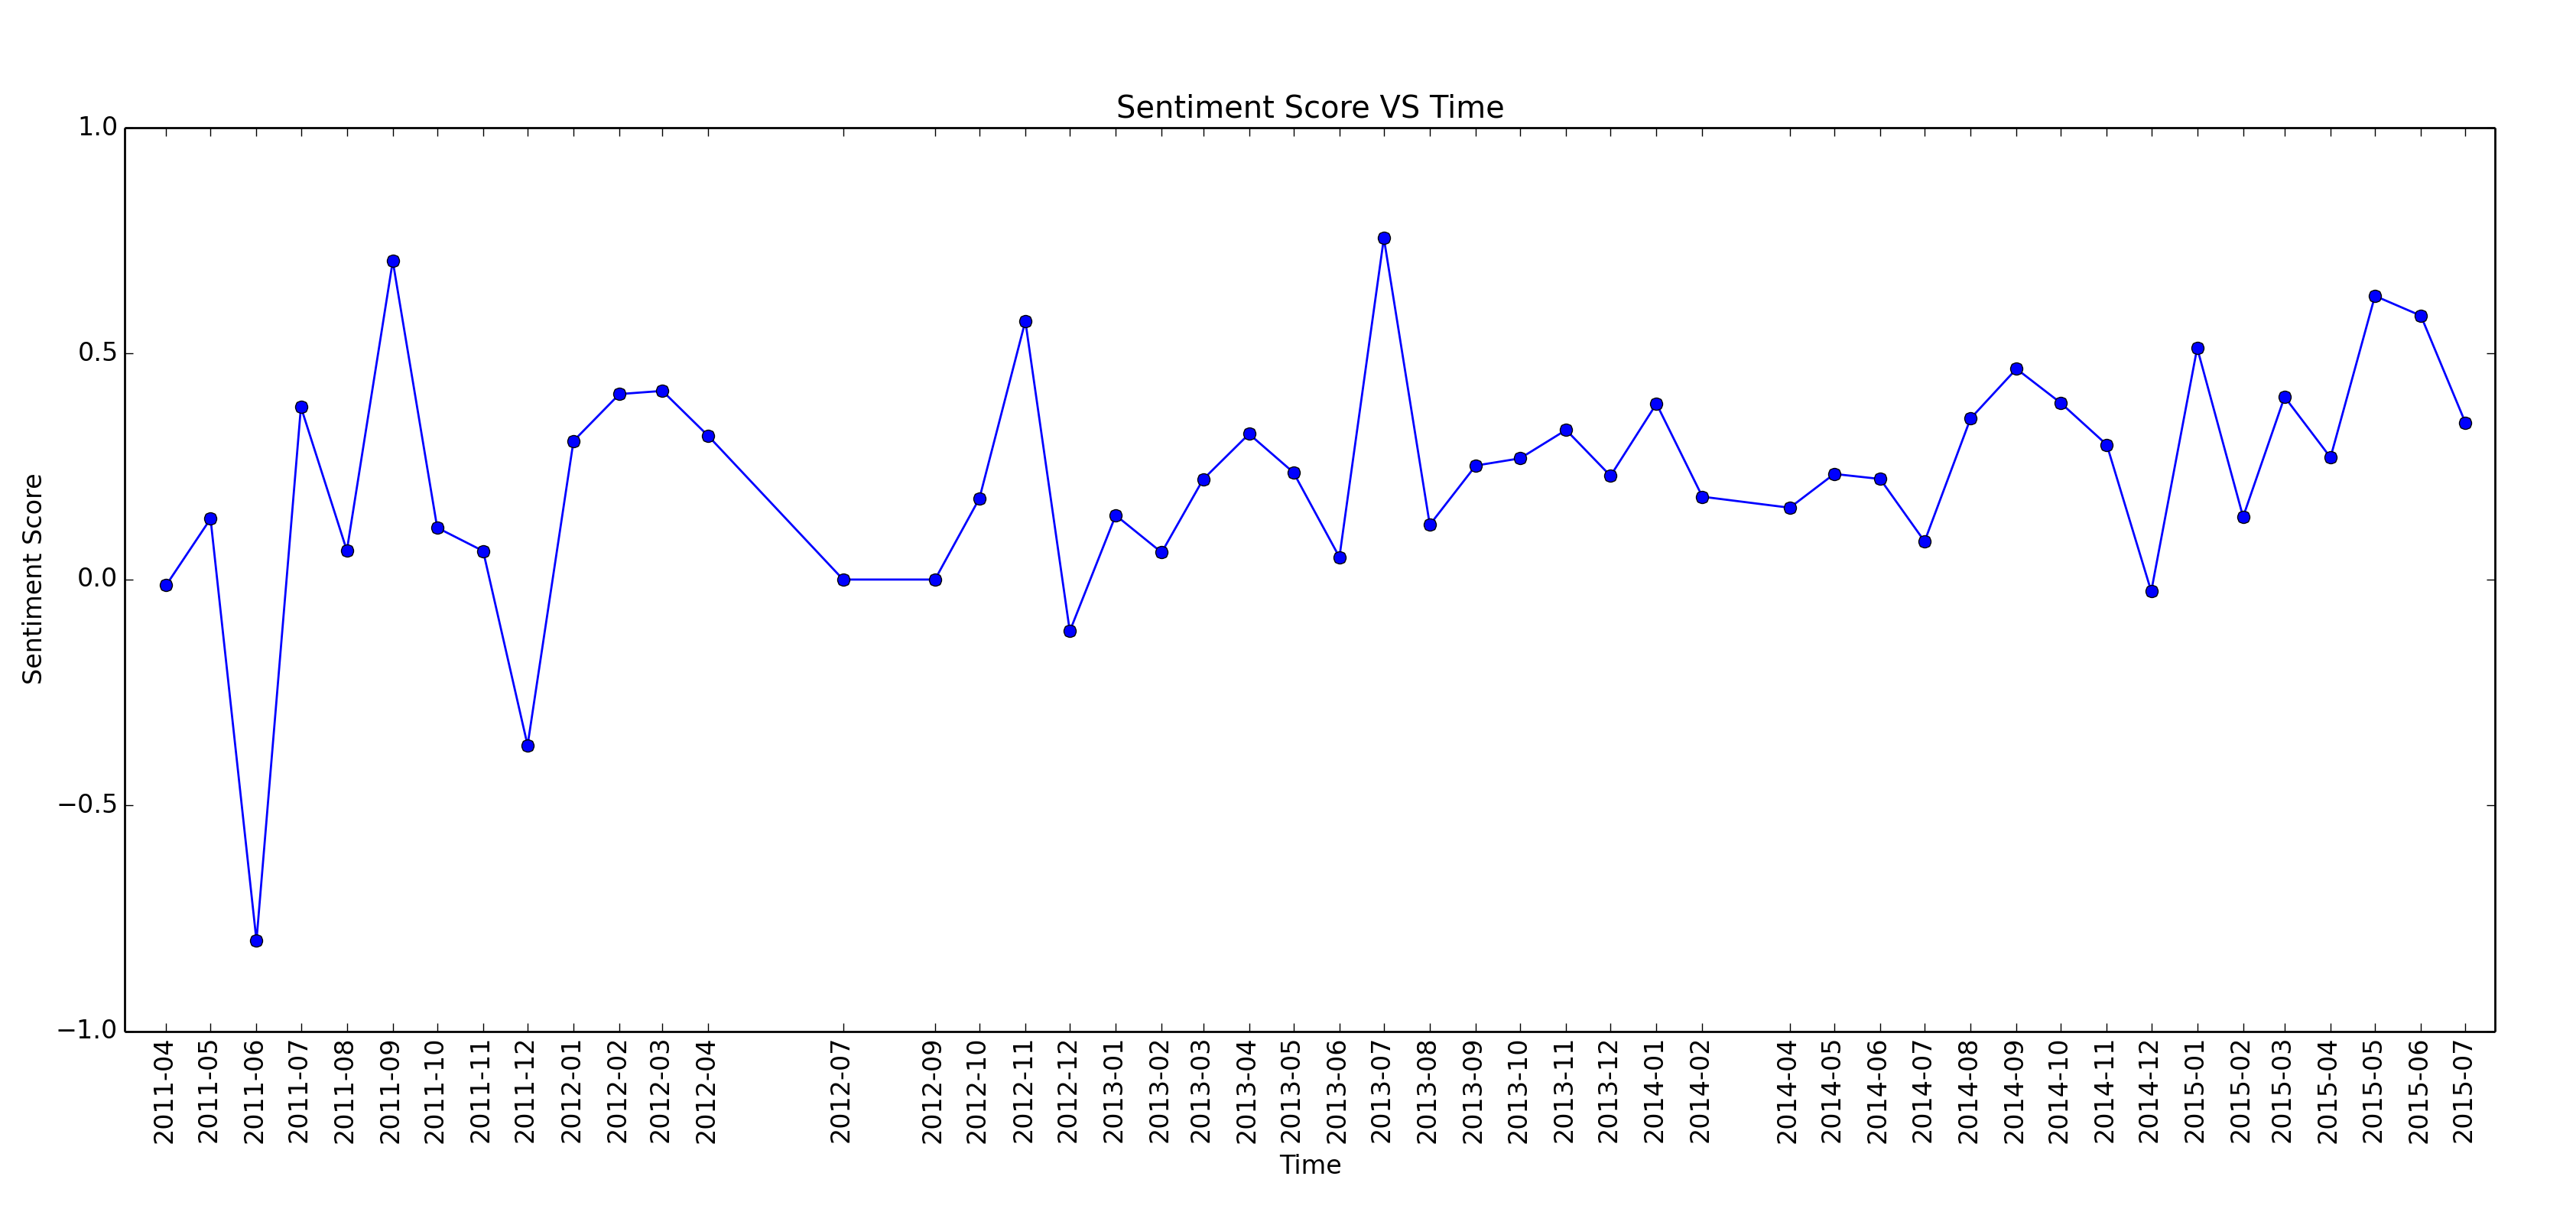
\includegraphics[width=550px, height=310px]{ponguru_senti_time}}
\end{center}
\newpage
thekiranbedi(Kiran Bedi)
\begin{center}
 \makebox[\textwidth]{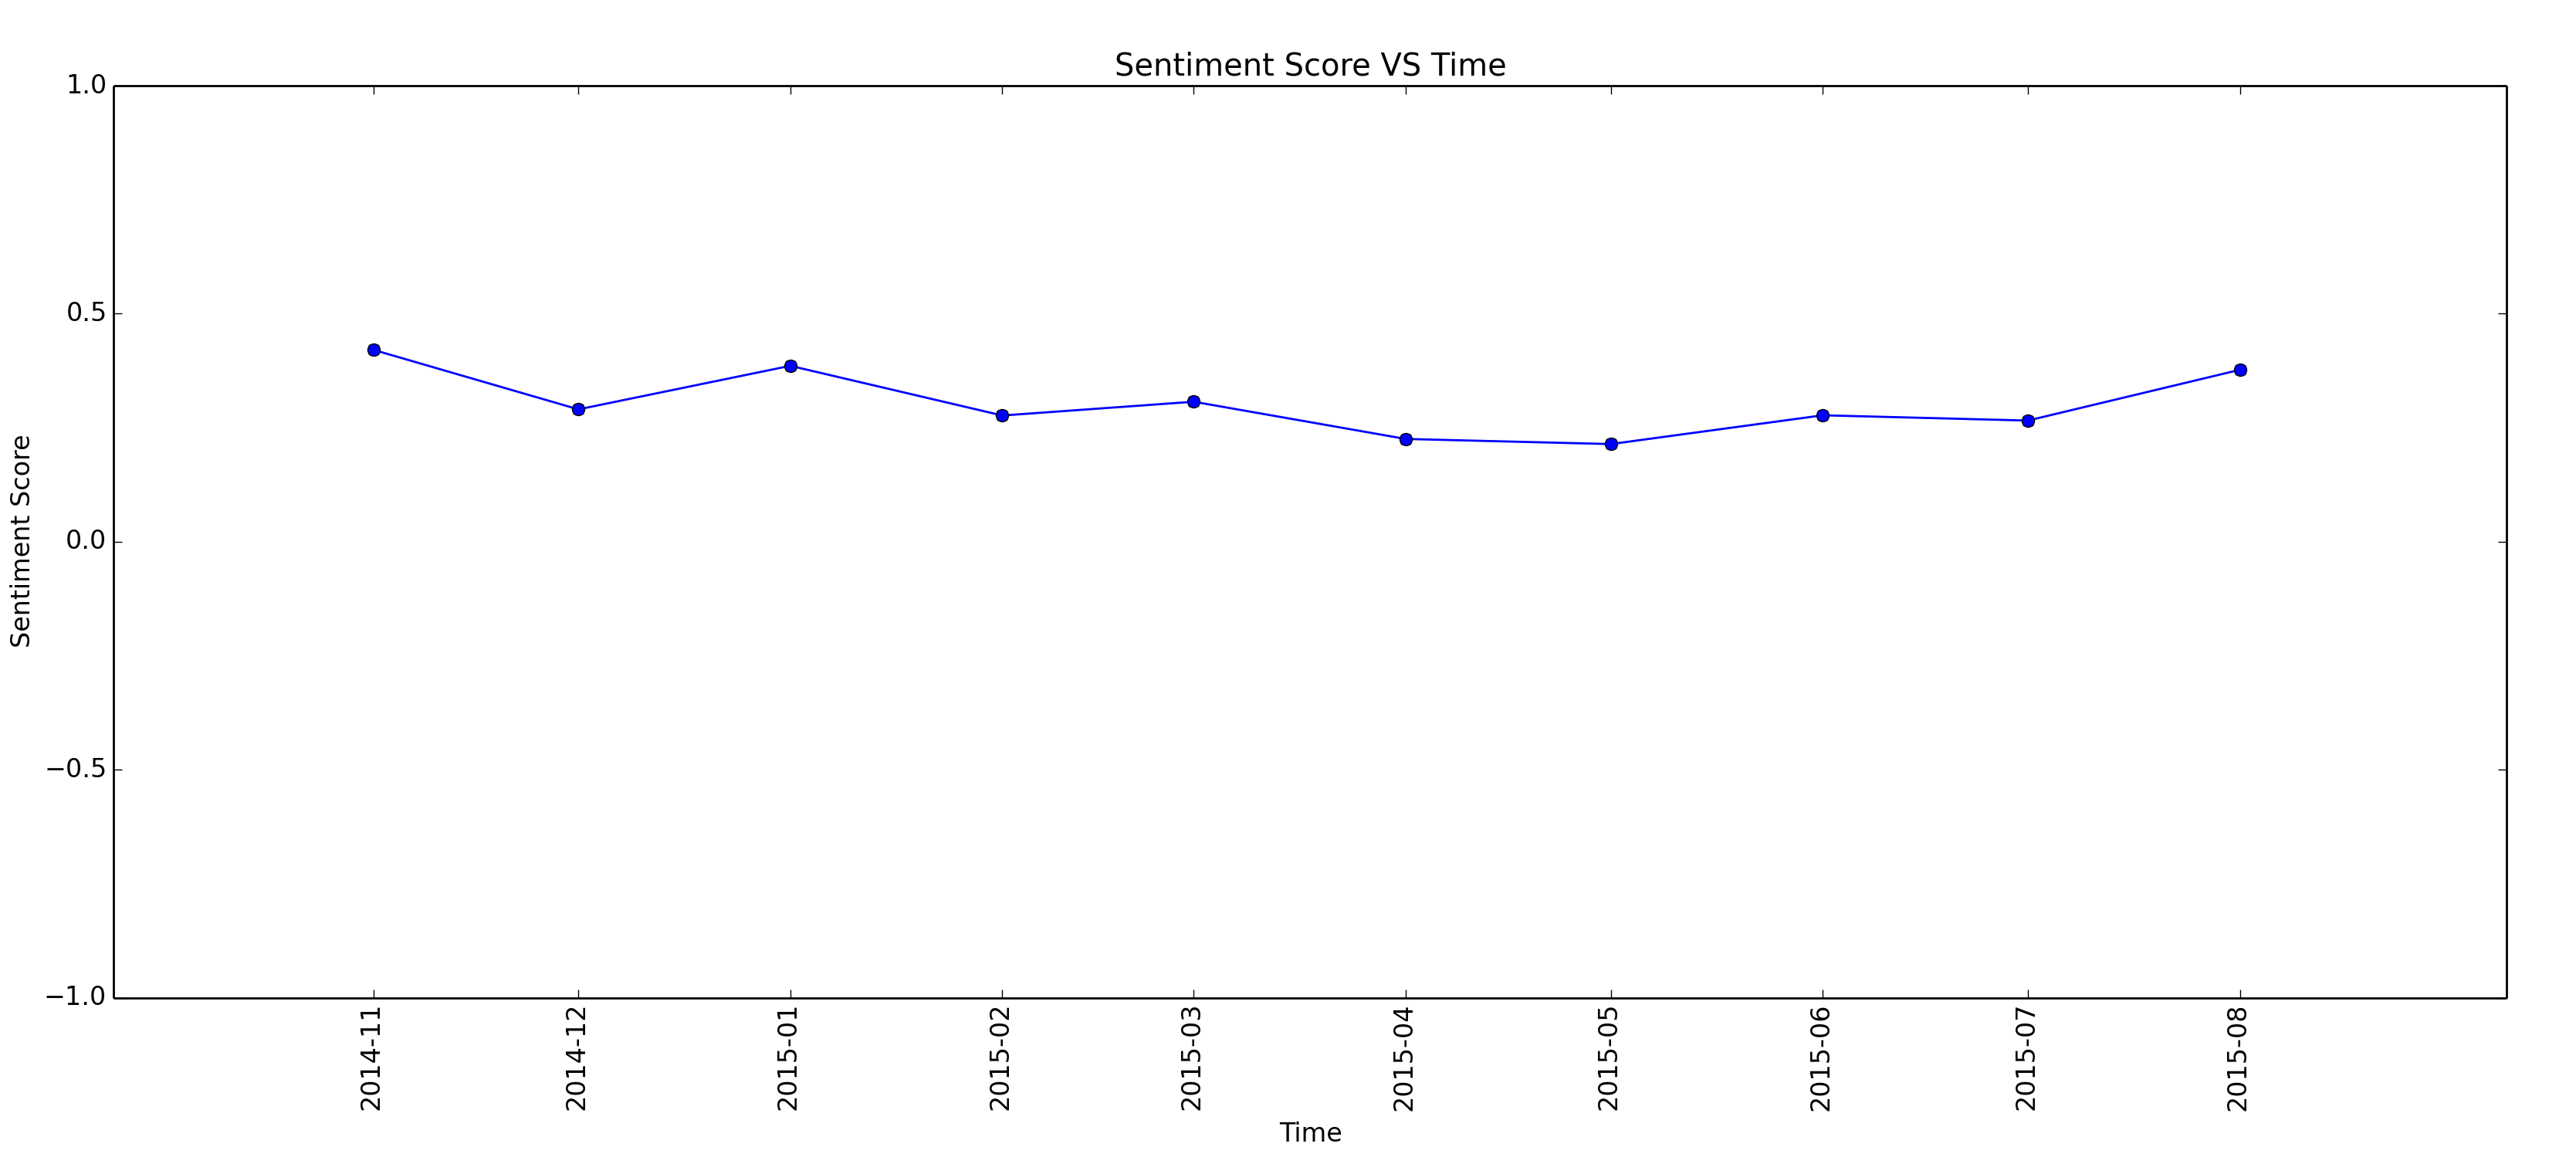
\includegraphics[width=550px, height=310px]{thekiranbedi_senti_time}}
\end{center}

\newpage
\subsection{Sentiment composition of tweets/posts of ID's}
Pie charts showing total sentiment composition of each ID's.\\
\begin{figure}[!htb]
\centering
\begin{tabular}{|c|c|c}
\hline
\subf{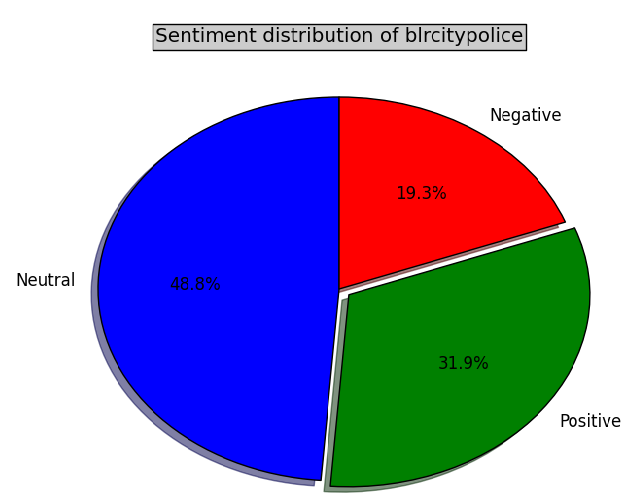
\includegraphics[width=130px,height=130px]{blrcitypolice_sentiment_dist}}
{}
&
\subf{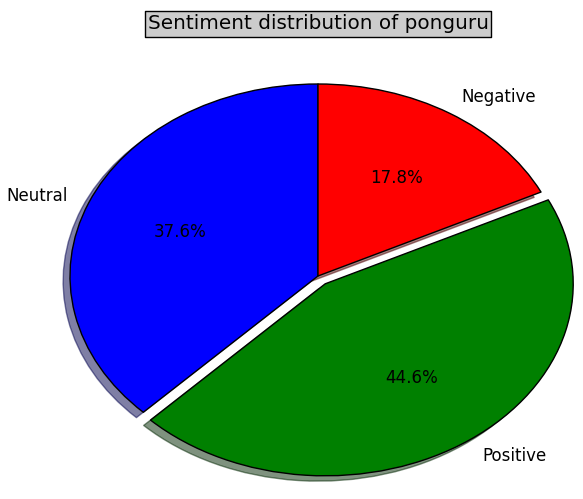
\includegraphics[width=130px,height=130px]{ponguru_sentiment_dist}}
{}
&
\subf{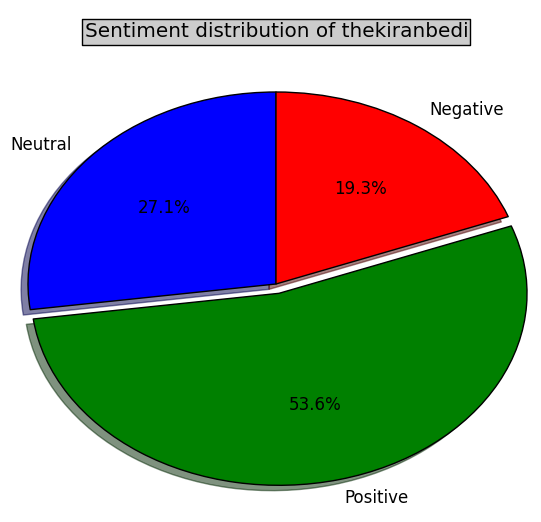
\includegraphics[width=130px,height=130px]{thekiranbedi_sentiment_dist}}
{}
\\
\hline
\end{tabular}
\end{figure}
\newpage
\subsection{Python program to get data from facebook for CERCatIIITD page. This program parses description in to What, Where and When components.}
\lstinputlisting[breaklines]{get-data.py}
\newpage
\subsection{Python program to get data from facebook for theblrcitypolice page. Store time, id, message and description in to mongo db for latter use.}
\lstinputlisting[breaklines]{get-data2.py}
\newpage
\subsection{A list file to be read by above two programs to get parameters for facebook graph API.}
\lstinputlisting[breaklines]{fb-data.list}
\newpage
\subsection{Python program to get data from twitter using Tweepy python library and twitter API and store it in mongo DB.}
\lstinputlisting[breaklines]{twitter-get-data.py}
\newpage
\subsection{Python program to generate graph of \#posts with time for all four IDs.}
\lstinputlisting[breaklines]{time_series_analaysis.py}
\newpage
\subsection{Python program to generate word clouds for the spikes and start month and end month of all the time series graph.}
\lstinputlisting[breaklines]{word_cloud_spikes.py}
\newpage
\subsection{Python program to generate word cloud for all the posts/tweets for all the IDs to get most frequent used words.}
\lstinputlisting[breaklines]{word_cloud.py}
\newpage
\subsection{Python program to get sentiment scores of posts/tweets in during a certain time period using Machpee community sentiment API and generate a CSV file.}
\lstinputlisting[breaklines]{sentiment_analysis2.py}
\newpage
\subsection{Python program to draw sentiment score for each day/month for all the IDs.}
\lstinputlisting[breaklines]{senti_time_series.py}
\newpage
\subsection{Python program to generate pie chart for sentiment composition of all the IDs.}
\lstinputlisting[breaklines]{darw_sentiment_pie.py}
\end{document}